\section{Results and discussion: The axial mass effect}
Figure~\ref{SKrates} displays the result of our calculation: ratios of the neutrino event rates caused by the QES interactions with hydrogen and oxygen nuclei in the Super-Kamiokande detector, evaluated with several values of conventional constant $M_{A}$ to ones computed with preliminary offered $M_{A}^{\mathrm{eff}}$. Figure~\ref{NOvArates} presents results for NO$\nu$A experiment in analogical way.

\begin{figure}[htb!]
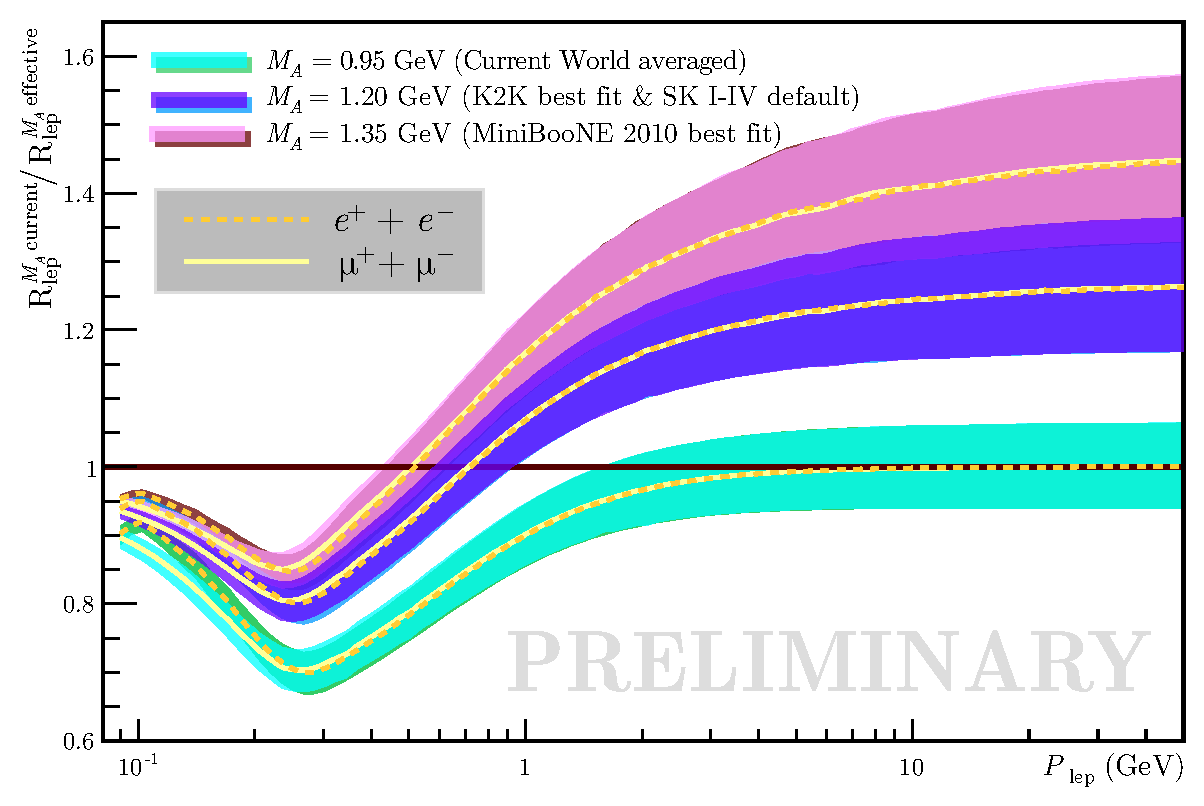
\includegraphics[width=\columnwidth]{./SK/cvsv2lmn_all2.eps}
\caption{\label{SKrates}Electron-like and muon-like event rates caused by the QES interactions in the Super-Kamiokande detector. The rates are evaluated with several constant values of $M_{A}$ and normalized to the rates calculated with $M_{A}^{\mathrm{eff}}$. The calculations are done for the normal neutrino mass hierarchy}
\end{figure}

\begin{figure}[htb!]
\begin{center}
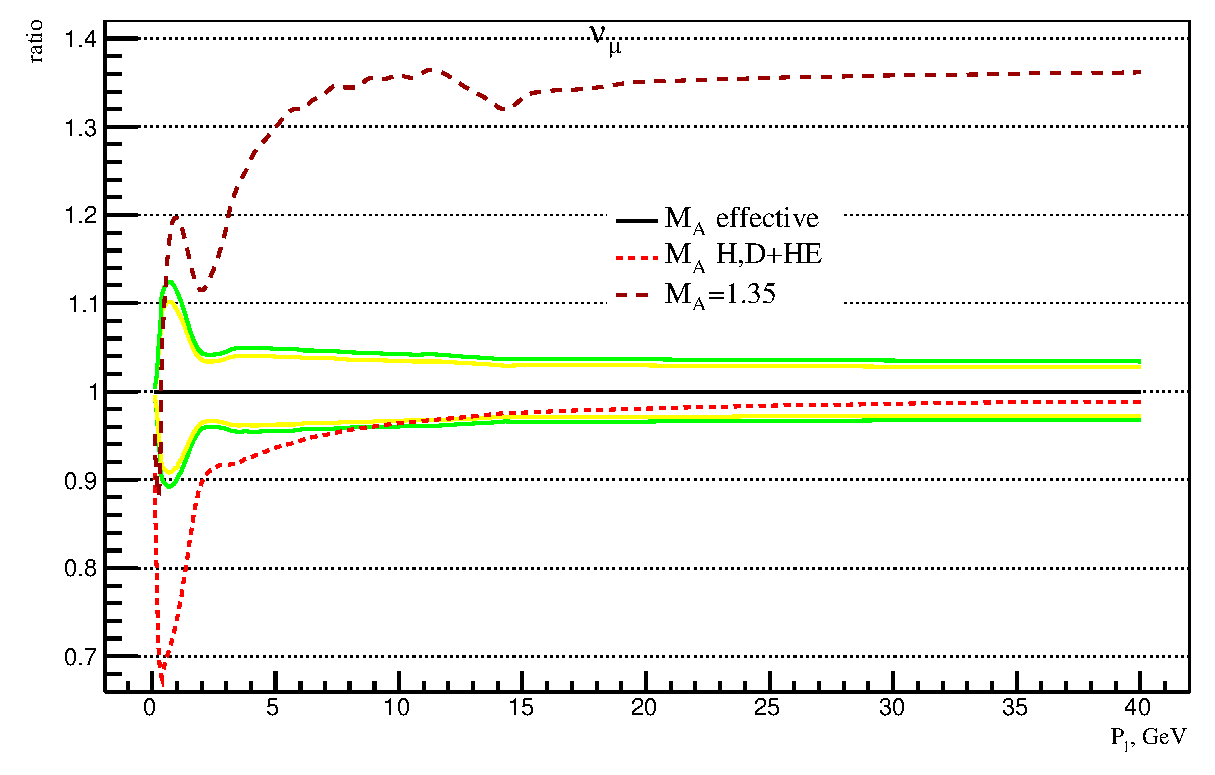
\includegraphics[width=0.9\columnwidth]{./NOvA/NOvA_newflux_Scintillator_nm_n5.eps}
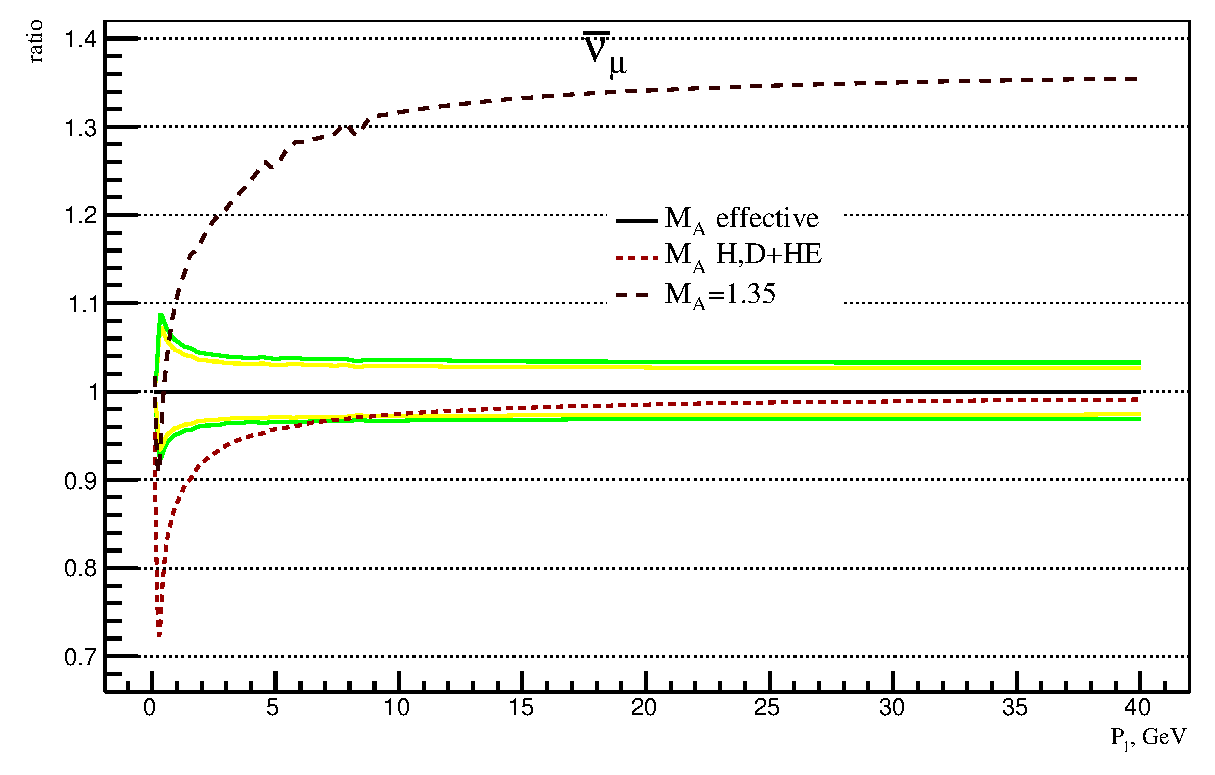
\includegraphics[width=0.9\columnwidth]{./NOvA/NOvA_newflux_Scintillator_am_n5.eps}
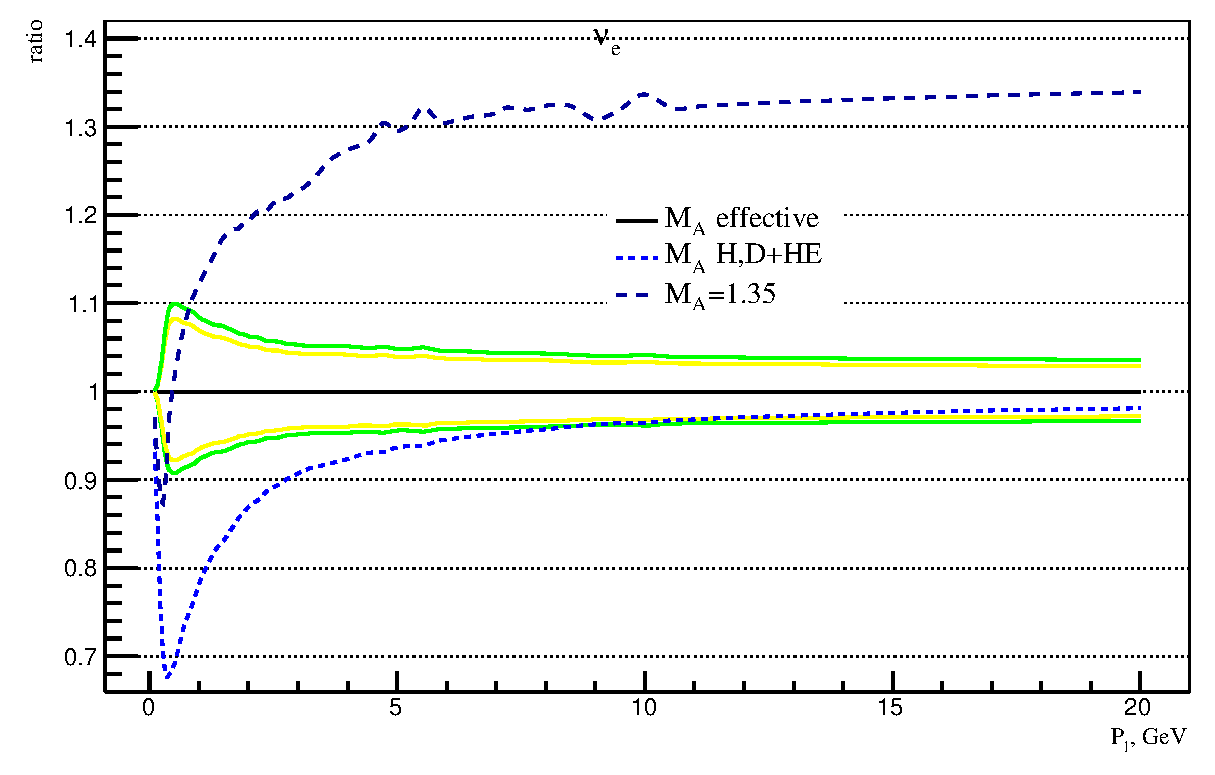
\includegraphics[width=0.9\columnwidth]{./NOvA/NOvA_newflux_Scintillator_ne_n5.eps}
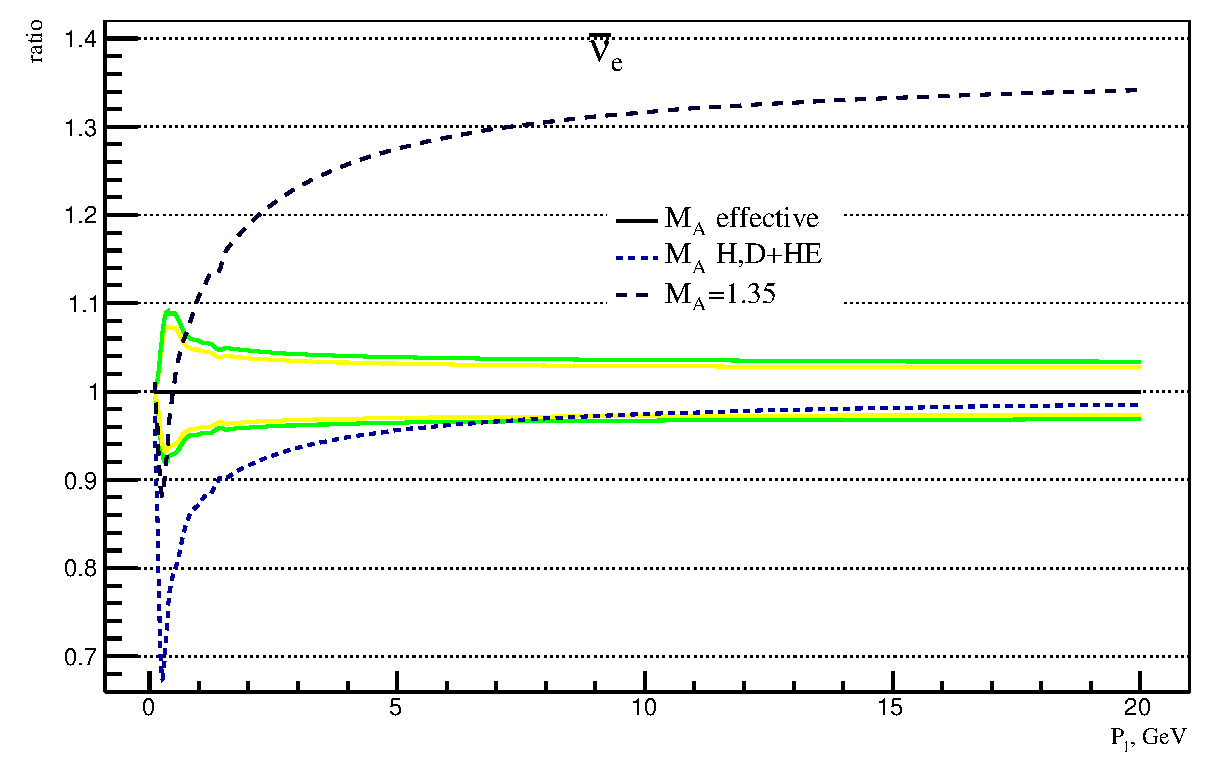
\includegraphics[width=0.9\columnwidth]{./NOvA/NOvA_newflux_Scintillator_ae_n5.eps}
\caption{\label{NOvArates}Charged lepton flux ratios in the Near Detector of NO$\nu$A experiment for $\nu$-beam mode calculated with $M_{A}$ obtained MiniBooNE experiment, deuterium best-fit $M_{A}$ value and with the effective nucleon axial mass}
\end{center}
\end{figure}

It can be seen, that the adequate choice of the axial mass value is very important to the neutrino event rate calculations: error in count rates predicted with high-energy and hydrogen/deuterium data near NO$\nu$A energy peak 2\,GeV achieves 6\%, using the MiniBooNE result $M_{A}=1.35$\,GeV~\cite{AguilarArevalo:2010zc} in high-energy region leads to approximately 30\% errors. Of course in experiments with two detectors this enormous uncertainty is roughly canceled out, but it affects experiment results through statictical uncertainties in fluxes. Because of the fact that effect depends on energy it cannot be eliminated by any renormalizing factor.

Figure~\ref{NOvAeffect} illustrates magnitude of the effect in comparison with $\nu_{\mu}\to{}\nu_{e}$ oscillation probability. Muon neutrino deficit in Far Detector, caused by oscillations to electron neutrino is comparable with deficit induced by using MiniBooNE value of $M_{A}$ at very low energies and significantly higher than one caused by exploiting best-fit deuterium $M_{A}$ value in whole energy range.

\begin{figure}[htb!]
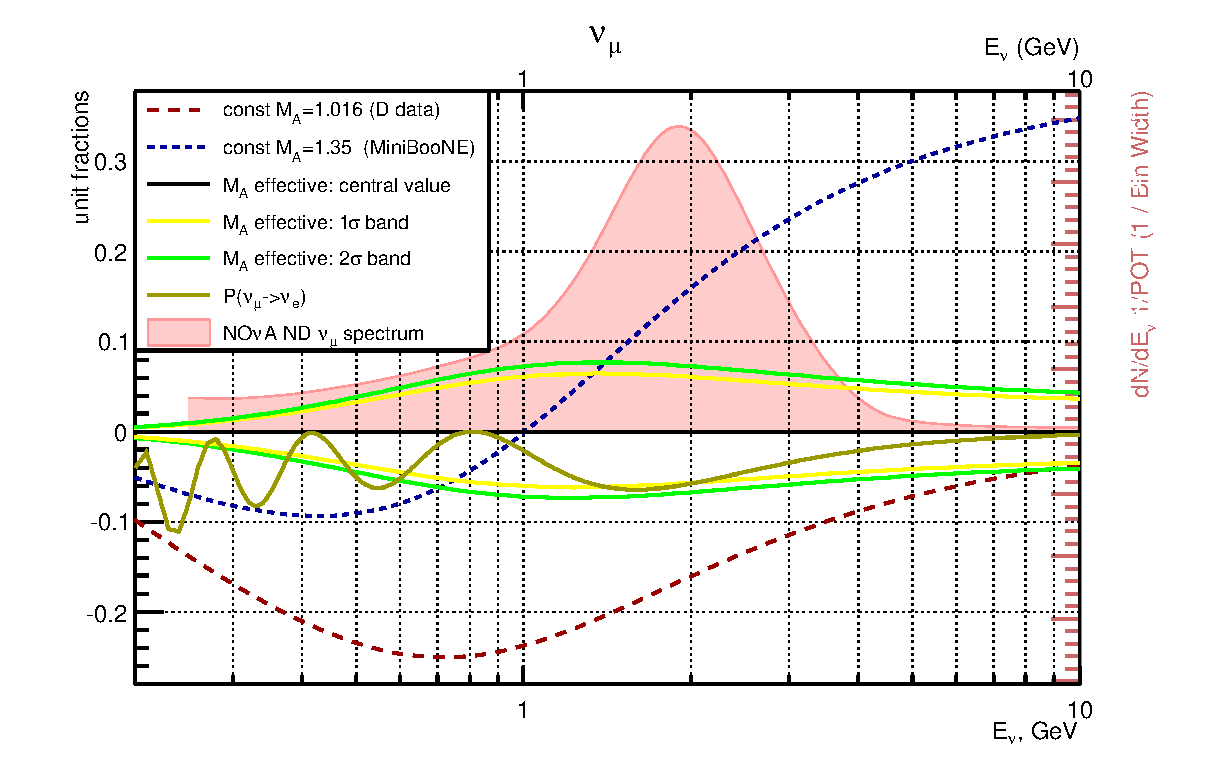
\includegraphics[width=\columnwidth]{./NOvA/Scintillator_nm_n5.eps}
\caption{\label{NOvAeffect}Comparison between $M_{A}^{\mathrm{eff}}$ impact to the total $\nu_{\mu}$ QES cross section and $P_{\nu_{\mu}\to{}\nu_{e}}$. $\nu_{\mu}$ spectrum in the Near Detector of NOvA in $\nu$-beam mode is drawn transparently in the same energy-axis for illustration}
\end{figure}

In Fig.~\ref{SKeffect} Super-Kamiokande electron-like fully-contained events mostly caused by quasielastic interactions are shown. It is seen that $M_{A}^{\mathrm{eff}}$ correction improve the agreement between MC prediction and experimental data points.

\begin{figure}[htb!]
\includegraphics[width=\columnwidth]{./SK/SK_effect_IH.eps}
\caption{\label{SKeffect}Electron-like fully-contained events in the Super-Kamiokande detector vs. lepton momentum. Blue (red) histogram corresponds to MC simulations of event rate with (without) oscillation effect. Purlpe rectangles represent blue histogram reweighed with effect of using $M_{A}^{\mathrm{eff}}$ instead of $M_{A}=1.2$\,GeV used in SK. The calculations are done for the inverse neutrino mass hierarchy}
\end{figure}

\begin{figure}[htb!]
\begin{center}
\includegraphics[width=0.9\columnwidth]{./SK/t23Ematne_11.eps}
\includegraphics[width=0.9\columnwidth]{./SK/t23Ematie_11.eps}
\includegraphics[width=0.9\columnwidth]{./SK/t23Ematnm_11.eps}
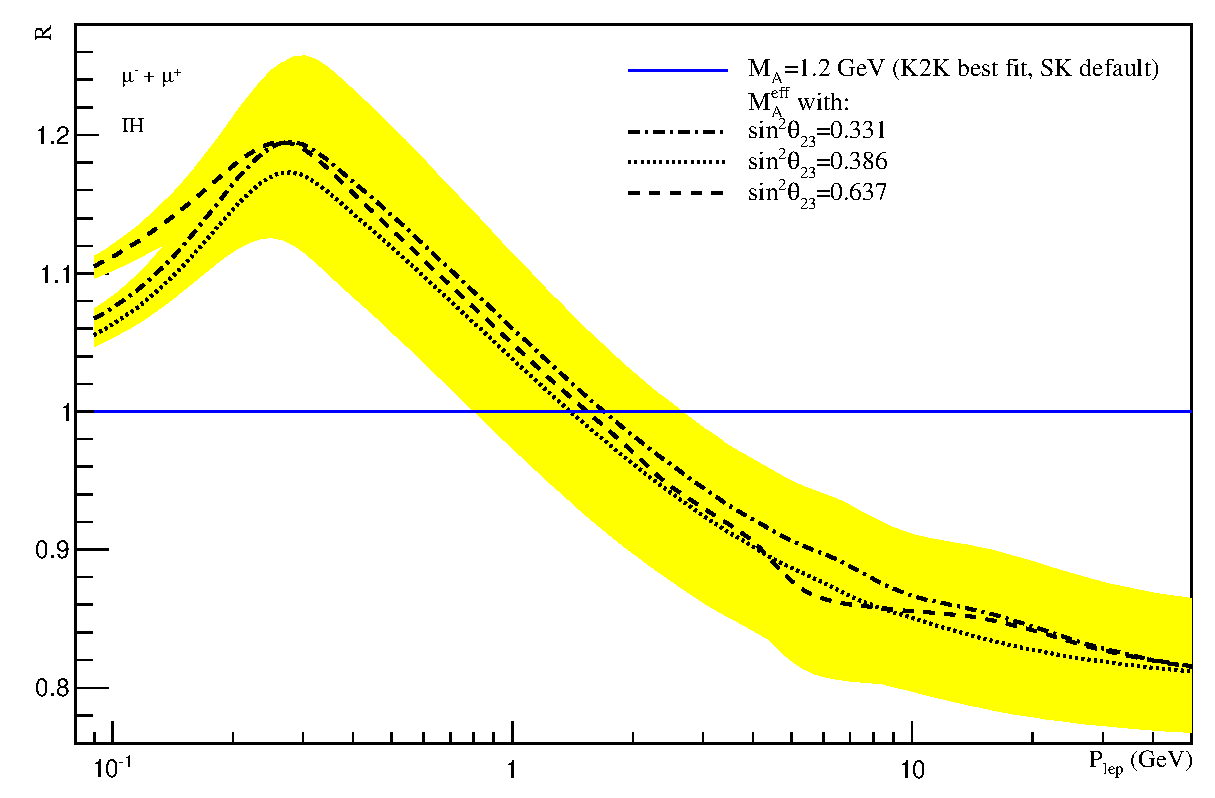
\includegraphics[width=0.9\columnwidth]{./SK/t23Ematim_11.eps}
\caption{\label{theta23}FIXME}
\end{center}
\end{figure}
